\documentclass[12pt,a4paper,titlepage,twoside]{article}
\usepackage[utf8]{inputenc}
\usepackage[spanish,es-noshorthands]{babel}
\usepackage{amsmath}
\usepackage{amsthm}
\usepackage{xcolor}
\usepackage{amsfonts}
\usepackage{amssymb}
\usepackage{graphicx}
\usepackage{lettrine}
\usepackage{color}
\usepackage{float}
\usepackage[top=2cm,bottom=4cm,outer=2cm,inner=2cm]{geometry}
\usepackage{fancybox}
\usepackage{tikz}
\usepackage{times}
\usepackage{verbatim}
\usetikzlibrary{arrows,shapes,positioning}
\usepackage{emptypage} % Para eliminar encabezado de las páginas en blanco
\usepackage{chngcntr}
\usepackage{etoolbox}
\usepackage{listings}
\usepackage[font={it,footnotesize},labelfont=bf]{caption}
\usepackage[colorlinks=true,linkcolor=black,urlcolor=black,citecolor=black]{hyperref}
\counterwithout{figure}{part}
\setlength\parindent{0pt} % Quita la indentación
\newtheorem{teorema}{Teorema}
\newcommand*{\autores}{
\begin{tabular}{r l}
GII+GIS: & Jesús Alcalde Alcázar \\
		 & Adrián Gutiérrez Jiménez\\
GIS:  	 & Carlos Vázquez Sánchez
\end{tabular}
}

%*******************************************************
%                 NO MODIFICAR
\newcommand*{\FSfont}[1]{%
  \fontencoding{T1}\fontfamily{#1}\selectfont}

\newlength{\tpheight}\setlength{\tpheight}{0.9\textheight}
\newlength{\txtheight}\setlength{\txtheight}{0.9\tpheight}
\newlength{\tpwidth}\setlength{\tpwidth}{0.9\textwidth}
\newlength{\txtwidth}\setlength{\txtwidth}{0.9\tpwidth}
\newlength{\drop}
%*******************************************************

% Crea una portada con los siguientes parámetros
%
% #1 : Título 
% #2 : Subtítulo
% #3 : Subsubtítulo
% #4 : Autor(es)
% #5 : Lugar
%

\newcommand*{\portada}[5]{
\begin{titlepage}
\begingroup
\vspace*{1cm}
\drop = 0.2\txtheight
\centering
\vfill
{\Huge \scshape #1}\\[\baselineskip]
{\Large \textbf{#2}}\\[\baselineskip]
{\Large \scshape #3}\\[\baselineskip]
\vspace*{0.3cm}
{\large \textit{#4}}\\[0.5\drop]

\includegraphics[scale=0.35]{./images/logoURJC.jpg}
\vspace*{1.5cm}

{\large \scshape #5, \today} \par
\begin{center}
\end{center}
\vfill\null
\endgroup
\end{titlepage}
}
 %*****************************************************
 

\makeatletter
\makeatother
\begin{document}
\portada{Investigación Operativa}{Práctica 2}{Teoría de Colas y Simulación}{\autores}{Móstoles}
\tableofcontents
\newpage{\ }

\section{Introducción}

En este documento se redacta el informe correspondiente al estudio y simulación de un \emph{``CallCenter''}, mendiante el cúal una empresa de telecominicaciones desea implantar un sistema de atención al cliente.\\

En primer lugar vamos a hacer un análisis de dicho sistema.

\subsection{Anális del escenario}
Éste sistema, según nos informa la compañía, puede recibir información a través de tres puntos y que cada uno de éstos es procesado de manera independiente:

\begin{itemize}
  \item \textbf{Llamadas por teléfono:} Se procesan en el \emph{``Servicio de tele-operadores''}. Tienen una media de llegadas de 15 llamadas por minuto ($\lambda_{1}$) y cada petición tarda una media de 15 segundos ($\mu_{1}$).
  \item \textbf{Peticiones vía Internet:} Se procesan mediante \emph{``Programas automáticos''}. Tienen una media de llegadas de 20 peticiones por minuto ($\lambda_{2}$) y cada petición tarda una media de 10 segundos ($\mu_{2}$).
  \item \textbf{Peticiones vía FAX:} Son procesadas por \emph{``Operadores de fax''}. Tienen una media de llegadas de 3 peticiones por minuto ($\lambda_{3}$) y cada petición tarda una media de 60 segundos ($\mu_{3}$).
\end{itemize}

Se explicita que las peticiones serán procesadas en orden de llegada y que esperaran en caso de que el servidor esté ocupado, por lo que suponemos que cada servidor dispone de una cola infinita para recibir peticiones.\\

Una vez que son procesados en los servidores mentados anteriormente, las peticiones se trasladas al servicio que corresponda, siguiendo una proporción similar, éstos son los servicios:

\begin{itemize}
  \item \textbf{Consultas sobre facturas:} Cada petición tiene un tiempo medio de servicio de 1 minuto ($\overline{X}_{4}$). Llegan hasta aquí el 80\% de las peticiones de cada servidor de llegadas más un 10\% de \emph{``reclamaciones de clientes''}.
  \item \textbf{Solicitudes de nuevos clientes:} Con un tiempo medio de servicio de 3 minutos ($\overline{X}_{5}$). Suponen el 10\% de las peticiones de cada servidor de llegadas.
  \item \textbf{Reclamaciones de clientes:} Se tardan 4 minutos de media en atender la petición ($\overline{X}_{6}$). Suponen el 2\% de las peticiones de cada servidor de llegadas.
  \item \textbf{Servicio tecnico :} Cada petición tiene un tiempo medio de servicio de 5 minutos ($\overline{X}_{7}$). Llegan hasta aquí el 8\% de las peticiones de cada servidor de llegadas más un 20\% de \emph{``reclamaciones de clientes''}.
\end{itemize}

\subsection{Representación visual del sistema}
Para poder entender mejor el sistema, con los datos proporcionados anteriormente, se ha esbozado el siguiente esquema del sistema utilizando un diagrama TQM (\emph{``Total Quality Management''}):

\tikzstyle{format} = [draw, thin, fill=blue!20]
\tikzstyle{medium} = [ellipse, draw, thin, fill=green!20, minimum height=2.5em]

\begin{figure}[H]
  \center{
  \begin{tikzpicture}[node distance=3cm, auto,>=latex', thick]

    \path[->] node (a1) {};
    \path[->] node[format, right of=a1] (s1) {Teléfono}
    (a1) edge node {$\lambda_{1}$} (s1);

    \path[->] node[below of=a1] (a2) {};
    \path[->] node[format, right of=a2] (s2) {Internet}
    (a2) edge node {$\lambda_{2}$} (s2);

    \path[->] node[below of=a2] (a3) {};
    \path[->] node[format, right of=a3] (s3) {FAX}
    (a3) edge node {$\lambda_{3}$} (s3);

    \path[->] node[format, right of=s1] (s4) {Facturas}
    (s1) edge node {1} (s4)
    (s2) edge node {2} (s4)
    (s3) edge node {3} (s4);

    \path[->] node[format, below of=s4] (s5) {Nuevos Clientes}
    (s1) edge node {1} (s5)
    (s2) edge node {2} (s5)
    (s3) edge node {3} (s5);

    \path[->] node[format, below of=s5] (s6) {Reclamaciones}
    (s1) edge node {1} (s6)
    (s2) edge node {2} (s6)
    (s3) edge node {3} (s6)
    (s6) edge node {4} (s5);

    \path[->] node[format, below of=s6] (s7) {Ser. Técnico}
    (s1) edge node {1} (s7)
    (s2) edge node {2} (s7)
    (s3) edge node {3} (s7)
    (s6) edge node {4} (s7);

  \end{tikzpicture}}
  \caption{Diagrama TQM del sistema}
\end{figure}

\section{Segunda parte}

\section{\textbf{\underline{Simulación y obtención de resultados}}}
Una vez realizados los cálculos teóricos, procedemos a crear un modelo de que represente el sistema indicado y simule su funcionamiento durante 24 horas. Para ellos se ha utilizado el software de INCONTROL \textit{Enterprise Dynamics}.\\ 
Una vez creado el modelo, simulamos 150 réplicas durante 24 horas, obteniendo los siguientes datos:\\\\
\textbf{Nota: }tanto los resultados mostrados directamente por \textit{Enterprise Dynamics} como los cálculos necesarios se adjuntan en el \textit{Anexo 2: Resultados simulación}
\subsection{Saturación servidores}
\begin{table}[H]
  \begin{center}
  \begin{tabular}{|c|c|}
    \hline
    \textbf{Servicio}       & \textbf{Nivel de saturación} \\ \hline
    Llamadas por Teléfono   & 75\%                   \\ \hline
    Peticiones por Internet & 83,25\%                  \\ \hline
    Peticiones por FAX      & 75\%                   \\ \hline
    Consulta Facturas      & 84,62\%                   \\ \hline
    Nuevos Clientes      & 81,38\%                   \\ \hline
    Reclamaciones      & 76\%                   \\ \hline
    Servicio Técnico      & 83,75\%                  \\ \hline
  \end{tabular}
\end{center}
  \caption{Nivel de saturación de cada servidor simulado}
  \end{table}
 \subsection{Tiempo medio de espera en las colas} 
  \begin{table}[H]
    \begin{center}
    \begin{tabular}{|c|c|}
      \hline
      \textbf{Cola}       & \textbf{Tiempo medio de espera (seg)} \\ \hline
      Llamadas por Teléfono   & 0                   \\ \hline
      Peticiones por Internet & 0                  \\ \hline
      Peticiones por FAX      & 0                   \\ \hline
      Consulta Facturas      & 0,01                   \\ \hline
      Nuevos Clientes      & 11,51                   \\ \hline
      Reclamaciones      & 67,93                   \\ \hline
      Servicio Técnico      & 17,16                  \\ \hline
    \end{tabular}
  \end{center}
    \caption{Tiempo medio de espera en cola simulado}
    \end{table}
    
  \subsection{Tiempo medio de respuesta para cada servicio}   
    \begin{table}[H]
      \begin{center}
      \begin{tabular}{|c|c|}
        \hline
        \textbf{Servicio}       & \textbf{Tiempo medio de respuesta (seg)} \\ \hline
        Llamadas por Teléfono   & 115.34                  \\ \hline
        Peticiones por Internet & 110.34                 \\ \hline
        Peticiones por FAX      & 160.34                   \\ \hline
      \end{tabular}
    \end{center}
      \caption{Tiempo medio de respuesta simulado}
      \end{table}
\section{\textbf{\underline{Conclusiones}}}
Tras la realización de este estudio podemos concluir que si se dispone de los operadores mínimos indicados anteriormente, el sistema es estable y la saturación de cada estación multiservicio no sobrepasa el 85\%, aunque el servidor de consultas sobre facturas tiene un muy pequeño margen de error al funcionar al 84,62\%. 


%  ANEXOS %
\newpage{\ }
\section{\textbf{\underline{ANEXO 1: Cálculos teóricos}}}
Uno de los requisitos especificados para la instalación del nuevo \emph{``Call Center''} es que los servidores tienen que tener una tasa de utilización inferior al 85\%. Para que esta condición se cumpla, ha de cumplirse que:

\begin{equation}
p \leq 0,85 \text{ \texttt{siendo:} }
p = \frac{\lambda_{n}}{m\mu_{n}} \text{ \texttt{y} } \mu_{n}= \frac{1}{\overline{X}_{n}}
\end{equation}

Para $m= numero\ de\ operadores$, $\mu_{n} = tasa\ de\ servicio\ n$, $\overline{X}_{n} = tiempo\ medio\ del\ servicio\ n$ y $\lambda_{n} = tasa\ de\ llegada\ del\ servicio\ n$.\\
Por lo que para calcular el número de operadores para cada servicio, basta con:

\begin{equation}
p = \frac{\lambda_{n}}{m\mu_{n}} \rightarrow p = \frac{\lambda_{n}\overline{X}_{n}}{m} \rightarrow m = \frac{\lambda_{n}\overline{X}_{n}}{p}
\end{equation}

\subsection{Cálculo de las ecuaciones de tráfico}
Para poder poner en práctica las formula anterior necesitamos saber las tasas de llegada de cada servicio. Para los tres primeros estos datos se corresponden con $\lambda_{1}$, $\lambda_{2}$ y $\lambda_{3}$, respectivamente.\\

Para los demás es necesario saber qué porcentaje de llegadas procede da cada lugar, quedándonos lo siguiente:

\begin{multline}\\
  I_{1} = \lambda_{1} \rightarrow I_{1} = 15 \\
  I_{2} = \lambda_{2} \rightarrow I_{2} = 20 \\
  I_{3} = \lambda_{3} \rightarrow I_{3} = 3 \\
  I_{4} = 0.8\cdot (I_{1}+I_{2}+I_{3}) + 0.1I_{6} \rightarrow I_{4} = 30.476 \\
  I_{5} = 0.1\cdot (I_{1}+I_{2}+I_{3})  \rightarrow I_{5} = 3.8 \\
  I_{6} = 0.02\cdot (I_{1}+I_{2}+I_{3})  \rightarrow I_{6} = 0.76 \\
  I_{7} = 0.08\cdot (I_{1}+I_{2}+I_{3})  \rightarrow I_{7} = 3.192 \\
  \end{multline}

Una vez con estos datos podemos calcular el número de operadores.

\subsection{Cálculo del número de operadores}
Eso significa que han de cumplirse estos valores:

\begin{multline}\\
  m_{1} = \frac{\lambda_{1}\overline{X}_{1}}{0.85} \rightarrow m_{1} = \frac{15\cdot 0.25}{0.85} \rightarrow m_{1} = 4.41 \\
  m_{2} = \frac{\lambda_{2}\overline{X}_{2}}{0.85} \rightarrow m_{2} = \frac{20\cdot 0.16}{0.85} \rightarrow m_{2} = 3.92\\
  m_{3} = \frac{\lambda_{3}\overline{X}_{3}}{0.85} \rightarrow m_{3} = \frac{3\cdot 1}{0.85} \rightarrow m_{3} = 3.52\\
  m_{4} = \frac{\lambda_{4}\overline{X}_{4}}{0.85} \rightarrow m_{4} = \frac{30.476\cdot 1}{0.85} \rightarrow m_{4} = 35.85\\
  m_{5} = \frac{\lambda_{5}\overline{X}_{5}}{0.85} \rightarrow m_{5} = \frac{3.8\cdot 3}{0.85} \rightarrow m_{5} = 13.41\\
  m_{6} = \frac{\lambda_{6}\overline{X}_{6}}{0.85} \rightarrow m_{6} = \frac{0.76\cdot 4}{0.85} \rightarrow m_{6} = 3.57\\
  m_{7} = \frac{\lambda_{7}\overline{X}_{7}}{0.85} \rightarrow m_{7} = \frac{3.192\cdot 5}{0.85} \rightarrow m_{7} = 18.77\\
\end{multline}

Como no se tratan de valores enteros y éstos deben de ser los valores mínimos, el número mínimo de operadores ha de ser:

\begin{table}[H]
  \begin{center}
  \begin{tabular}{|c|c|}
    \hline
    \textbf{Servicio}       & \textbf{Operadores} \\ \hline
    Llamadas por Teléfono   & 5                   \\ \hline
    Peticiones por Internet & 4                   \\ \hline
    Peticiones por FAX      & 4                   \\ \hline
    Consulta Facturas      & 36                   \\ \hline
    Nuevos Clientes      & 14                   \\ \hline
    Reclamaciones      & 4                   \\ \hline
    Servicio Técnico      & 19                   \\ \hline
  \end{tabular}
\end{center}
  \caption{Numero de operadores mínimos para lograr una tasa de utilización inferior al 85\%}
\end{table}

\subsection{Cálculo de la tasa de uso de cada servidor}
Como ya se ha indicado anteriormente, la tasa de uso de cada servidor la obtenemos mediante la fórmula:
\begin{equation}
p = \frac{\lambda_{n}}{m\mu_{n}}
\end{equation}
Por tanto, insertamos el número de operarios necesarios calculados y obtenemos la tasa de uso de cada servidor:
\begin{multline}\\
p_{1} = \frac{\lambda_{1}}{m_{1}\mu_{1}} = \frac{15}{5\times 4} = 0,75 \\
p_{2} = \frac{\lambda_{2}}{m_{2}\mu_{2}} = \frac{20}{4\times 6} = 0,8\\
p_{3} = \frac{\lambda_{3}}{m_{3}\mu_{3}} = \frac{3}{4\times 1} = 0,75\\
p_{4} = \frac{\lambda_{4}}{m_{4}\mu_{4}} = \frac{30,476}{36\times 1} = 0,8465\\
p_{5} = \frac{\lambda_{5}}{m_{5}\mu_{5}} = \frac{3,8}{14\times 0,33} = 0,8225\\
p_{6} = \frac{\lambda_{6}}{m_{6}\mu_{6}} = \frac{0,76}{4\times 0,25} = 0,75\\
p_{7} = \frac{\lambda_{7}}{m_{7}\mu_{7}} = \frac{3,192}{19\times 0,2} = 0,84\\
\end{multline}
Los resultados los agrupamos en la siguiente tabla:
\begin{table}[H]
  \begin{center}
  \begin{tabular}{|c|c|}
    \hline
    \textbf{Servicio}       & \textbf{Tasa de uso} \\ \hline
    Llamadas por Teléfono   & 75\%                   \\ \hline
    Peticiones por Internet & 80\%                  \\ \hline
    Peticiones por FAX      & 75\%                   \\ \hline
    Consulta Facturas      & 84,65\%                   \\ \hline
    Nuevos Clientes      & 82,25\%                   \\ \hline
    Reclamaciones      & 75\%                   \\ \hline
    Servicio Técnico      & 84\%                  \\ \hline
  \end{tabular}
\end{center}
  \caption{Tasa de uso de cada servidor}
  \end{table}
\subsection{Cálculo del tiempo medio de respuesta en cada servidor}

El tiempo medio de espera se calcula utilizando la siguiente fórmula:

\begin{equation}
\overline{R}_{i} = \frac{1}{m_{i}\mu_{i}-I_{i}}
\end{equation}

Siendo $i$ el servidor.\\

Sustituyendo en la formula obtenemos los siguientes resultados:

\begin{multline}\\
\overline{R}_{1} = \frac{1}{m_{1}\mu_{1}-I_{1}} = \frac{1}{5\times 4 - 15} = 0,2\\
\overline{R}_{2} = \frac{1}{m_{2}\mu_{2}-I_{2}} = \frac{1}{4\times 6 - 20} = 0,25\\
\overline{R}_{3} = \frac{1}{m_{3}\mu_{3}-I_{3}} = \frac{1}{4\times 1 - 3} = 1\\
\overline{R}_{4} = \frac{1}{m_{4}\mu_{4}-I_{4}} = \frac{1}{36\times 1 - 30,48} = 0,18\\
\overline{R}_{5} = \frac{1}{m_{5}\mu_{5}-I_{5}} = \frac{1}{14\times 0,33 - 3,8} = 0,82\\
\overline{R}_{6} = \frac{1}{m_{6}\mu_{6}-I_{6}} = \frac{1}{4\times 0,25 - 0,76} = 4,17\\
\overline{R}_{7} = \frac{1}{m_{7}\mu_{7}-I_{7}} = \frac{1}{18\times 0,2 - 3,04} = 1,79\\
\end{multline}
Los resultados los agrupamos en la siguiente tabla:

\begin{table}[H]
  \begin{center}
  \begin{tabular}{|c|c|}
    \hline
    \textbf{Servicio}       & \textbf{Tiempo medio de espera en cada servidor(m)} \\ \hline
    Llamadas por Teléfono   & 0,2                   \\ \hline
    Peticiones por Internet & 0,1                  \\ \hline
    Peticiones por FAX      & 1                   \\ \hline
    Consulta Facturas      & 0,18                   \\ \hline
    Nuevos Clientes      & 0,82                   \\ \hline
    Reclamaciones      & 4,17                   \\ \hline
    Servicio Técnico      & 1,79                   \\ \hline
  \end{tabular}
\end{center}
  \caption{Tiempo medio de espera en cada servidor}
  \end{table}
  
\subsection{Cálculo del tiempo medio de respuesta para cada tipo de trabajo}
El tiempo medio de respuesta para cada tipo de trabajo se calcula multiplicando el tiempo medio de espera de cada servidor por la probabilidad de que la solicitud pase por dicho servidor.\\

Es decir:
\begin{multline}\\
\overline{R}' = \overline{R}_{1} + 0,8\overline{R}_{4} + 0,1\overline{R}_{5} + 0,02\overline{R}_{6} + 0,08\overline{R}_{7} + 0,02\times 0,1\overline{R}_{4} + 0,02\times 0,2\overline{R}_{7} = 0,66\\
\overline{R}'' = \overline{R}_{2} + 0,8\overline{R}_{4} + 0,1\overline{R}_{5} + 0,02\overline{R}_{6} + 0,08\overline{R}_{7} + 0,02\times 0,1\overline{R}_{4} + 0,02\times 0,2\overline{R}_{7} = 0,71\\
\overline{R}''' = \overline{R}_{3} + 0,8\overline{R}_{4} + 0,1\overline{R}_{5} + 0,02\overline{R}_{6} + 0,08\overline{R}_{7} + 0,02\times 0,1\overline{R}_{4} + 0,02\times 0,2\overline{R}_{7} = 1,46\\
\end{multline}

\subsection{Cálculo del tiempo medio de espera total}
El tiempo medio de respuesta total se calcula mediante la siguiente fórmula:

\begin{equation}
\overline{R}_{T} = \frac{\lambda_{1}}{\lambda_{1}+\lambda_{2}+\lambda_{3}}\times \overline{R}' + \frac{\lambda_{2}}{\lambda_{1}+\lambda_{2}+\lambda_{3}}\times \overline{R}'' + \frac{\lambda_{3}}{\lambda_{1}+\lambda_{2}+\lambda_{3}}\times \overline{R}'''
\end{equation}

Sustituyendo obtenemos el siguiente resultado:

\begin{equation}
\overline{R}_{T} = \frac{15}{15+20+3}\times 0,66 + \frac{20}{15+20+3}\times 0,71 + \frac{3}{15+20+3}\times 1,46 = 0,75
\end{equation}

\subsection{Cálculo del tiempo medio de espera en cada servidor}
El tiempo medio de espera se calcula según la siguiente fórmula:

\begin{equation}
\overline{W}_{i} = \overline{R}_{i} - \overline{X}_{i}
\end{equation}

Debido a que ya no existe un único operador por cada servidor, sino que hay $m_{i}$ operadores quedaría de la siguiente forma:

\begin{equation}
\overline{W}_{i} = \overline{R}_{i} - \frac{\overline{X}_{i}}{m_{i}}
\end{equation}

Sustituyendo en la fórmula anterior obtenemos los siguientes resultados:

\begin{multline}\\
\overline{W}_{1} = \overline{R}_{1} - \frac{\overline{X}_{1}}{m_{1}} = 0,2 - \frac{0,25}{5} = 0,15\\
\overline{W}_{2} = \overline{R}_{2} - \frac{\overline{X}_{2}}{m_{2}} = 0,25 - \frac{0,17}{4} = 0,21\\
\overline{W}_{3} = \overline{R}_{3} - \frac{\overline{X}_{3}}{m_{3}} = 1 - \frac{1}{4} = 0,75\\
\overline{W}_{4} = \overline{R}_{4} - \frac{\overline{X}_{4}}{m_{4}} = 0,18 - \frac{1}{36} = 0,15\\
\overline{W}_{5} = \overline{R}_{5} - \frac{\overline{X}_{5}}{m_{5}} = 0,82 - \frac{3}{14} = 0,61\\
\overline{W}_{6} = \overline{R}_{6} - \frac{\overline{X}_{6}}{m_{6}} = 4,17 - \frac{4}{4} = 3,17\\
\overline{W}_{7} = \overline{R}_{7} - \frac{\overline{X}_{7}}{m_{7}} = 1,79 - \frac{5}{18} = 1,51\\
\end{multline}
\section{\textbf{\underline{ANEXO 2: Resultados simulación}}}
La simulación realizada en el software de INCONTROL \textit{Enterprise Dynamics} se ha realizado sobre todo el sistema, durrante 24 horas y con 150 réplicas. A continuación se adjuntan los resultados obtenidos:

\begin{figure}[H]
\begin{center}
\centering
  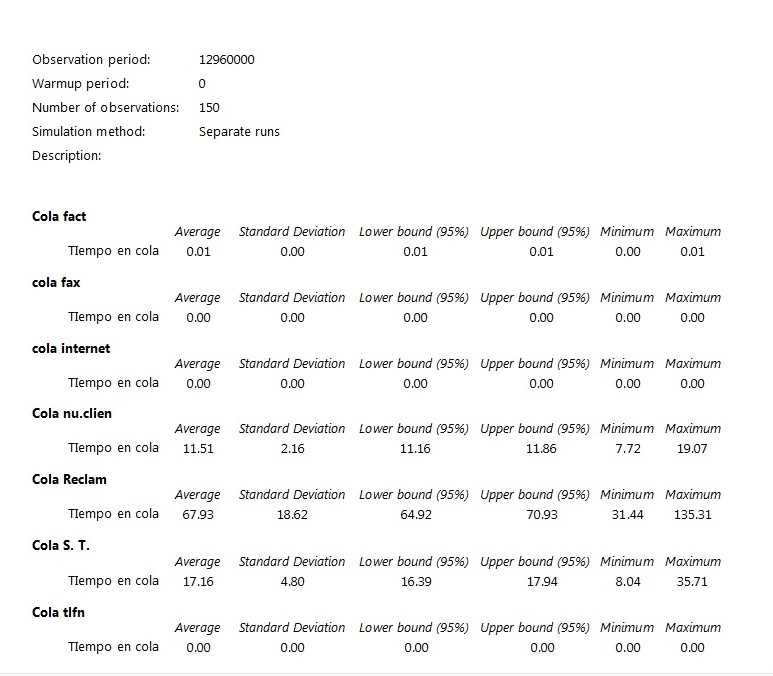
\includegraphics[width=1\textwidth]{./images/foto1}
  \caption{Resultados de la simulación 1}
  \label{fig: Resultados de la simulacion 1}
\end{center}
\end{figure}
\begin{figure}[H]
\begin{center}
\centering
  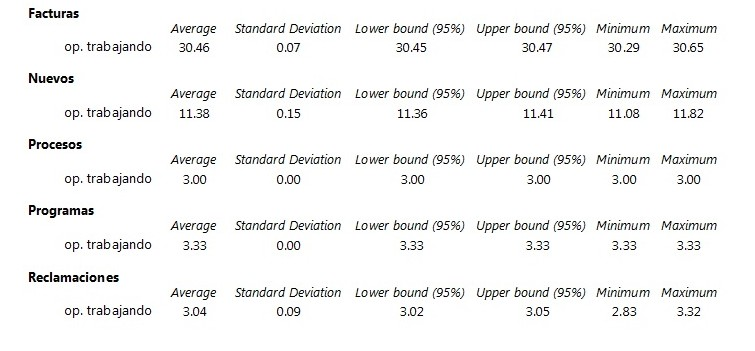
\includegraphics[width=1\textwidth]{./images/foto2}
  \caption{Resultados de la simulación 2}
  \label{fig: Resultados de la simulacion 2}
\end{center}
\end{figure}
\begin{figure}[H]
\begin{center}
\centering
  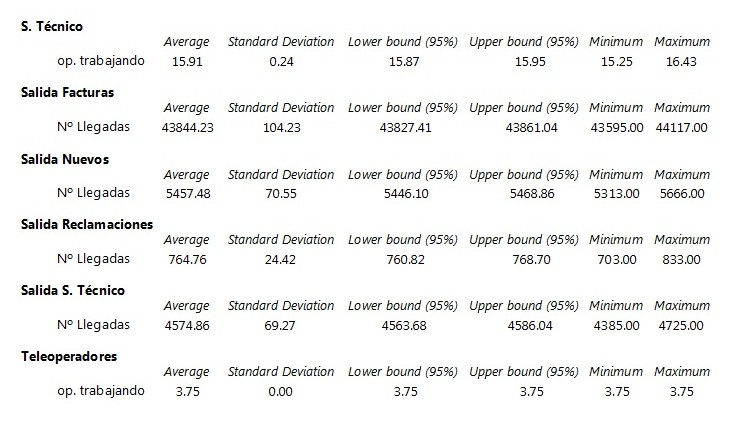
\includegraphics[width=1\textwidth]{./images/foto3}
  \caption{Resultados de la simulación 3}
  \label{fig: Resultados de la simulacion 3}
\end{center}
\end{figure}
Por tanto, podemos obtener directamente el tiempo medio de espera en cada cola, así como el tráfico que pasa por cada servidor. Para calcular la saturación del servidor basta con obtener el cociente entre el número medio de servidores activos obtenidos en la simulación ($X_{i}$) y el número de operarios totales para cada servidor $i$ ($op.s_{i}$):
\begin{multline}\\
p_{1 simulado} = \frac{X_{1}}{op.s_{1}} = \frac{3,75}{5} = 0,75 \\
p_{2 simulado} = \frac{X_{2}}{op.s_{2}} = \frac{3,33}{4} = 0,832\\
p_{3 simulado} = \frac{X_{3}}{op.s_{3}} = \frac{3}{4} = 0,75\\
p_{4 simulado} = \frac{X_{4}}{op.s_{4}} = \frac{30,46}{36} = 0,846\\
p_{5 simulado} = \frac{X_{5}}{op.s_{5}} = \frac{11,38}{14} = 0,813\\
p_{6 simulado} = \frac{X_{6}}{op.s_{6}} = \frac{3,04}{4} = 0,76\\
p_{7 simulado} = \frac{X_{7}}{op.s_{7}} = \frac{15,91}{19} = 0,837\\
\end{multline}

Además podemos saber el tiempo medio de espera para cada tipo de petición ya que conocemos el tiempo medio de espera en cada servidor, así como en su cola:
\begin{multline}\\
\overline{R}_{tlfn} = cola\_tlfn + \overline{X}_{1} + 0.8(cola\_facturas+\overline{X}_{4}) +\\ 0.1(cola\_nuevos+\overline{X}_{5}) + 0.02(cola\_reclamaciones+\overline{X}_{6}) + 0.08(cola\_s.tecnico+\overline{X}_{7})\\ + 0.02*0.1(cola\_facturas+\overline{X}_{4}) + 0.02*0.2(cola\_s.tecnico+\overline{X}_{7}) =\\
0+15+0.8(0.01+60)+ 0.1(11.51+180) + 0.02(67.93+240) + 0.08(17.16+300) \\+ 0.02*0.1(11.51+180) + 0.02*0.2(17.16+300)\\
=115.34 \\
\end{multline}
Obtener los dos restantes tiempos medios de respuesta es similar al calculado anteriormente, pero cambiando $cola\_tlfn + \overline{X}_{1}$ por $cola\_internet + \overline{X}_{2}$ y $cola\_fax + \overline{X}_{3}$. respectivamente:
\begin{multline}\\
\overline{R}_{internet} = 110.34 \\
\overline{R}_{fax} = 160.34 \\
\end{multline}



\end{document}
